\documentclass[11pt,preprint]{elsarticle}

\usepackage{lmodern}
%%%% My spacing
\usepackage{setspace}
\setstretch{1.2}
\DeclareMathSizes{12}{14}{10}{10}

% Wrap around which gives all figures included the [H] command, or places it "here". This can be tedious to code in Rmarkdown.
\usepackage{float}
\let\origfigure\figure
\let\endorigfigure\endfigure
\renewenvironment{figure}[1][2] {
    \expandafter\origfigure\expandafter[H]
} {
    \endorigfigure
}

\let\origtable\table
\let\endorigtable\endtable
\renewenvironment{table}[1][2] {
    \expandafter\origtable\expandafter[H]
} {
    \endorigtable
}


\usepackage{ifxetex,ifluatex}
\usepackage{fixltx2e} % provides \textsubscript
\ifnum 0\ifxetex 1\fi\ifluatex 1\fi=0 % if pdftex
  \usepackage[T1]{fontenc}
  \usepackage[utf8]{inputenc}
\else % if luatex or xelatex
  \ifxetex
    \usepackage{mathspec}
    \usepackage{xltxtra,xunicode}
  \else
    \usepackage{fontspec}
  \fi
  \defaultfontfeatures{Mapping=tex-text,Scale=MatchLowercase}
  \newcommand{\euro}{€}
\fi

\usepackage{amssymb, amsmath, amsthm, amsfonts}

\def\bibsection{\section*{References}} %%% Make "References" appear before bibliography


\usepackage[numbers]{natbib}

\usepackage{longtable}
\usepackage[margin=2.3cm,bottom=2cm,top=2.5cm, includefoot]{geometry}
\usepackage{fancyhdr}
\usepackage[bottom, hang, flushmargin]{footmisc}
\usepackage{graphicx}
\numberwithin{equation}{section}
\numberwithin{figure}{section}
\numberwithin{table}{section}
\setlength{\parindent}{0cm}
\setlength{\parskip}{1.3ex plus 0.5ex minus 0.3ex}
\usepackage{textcomp}
\renewcommand{\headrulewidth}{0.2pt}
\renewcommand{\footrulewidth}{0.3pt}

\usepackage{array}
\newcolumntype{x}[1]{>{\centering\arraybackslash\hspace{0pt}}p{#1}}

%%%%  Remove the "preprint submitted to" part. Don't worry about this either, it just looks better without it:
\makeatletter
\def\ps@pprintTitle{%
  \let\@oddhead\@empty
  \let\@evenhead\@empty
  \let\@oddfoot\@empty
  \let\@evenfoot\@oddfoot
}
\makeatother

 \def\tightlist{} % This allows for subbullets!

\usepackage{hyperref}
\hypersetup{breaklinks=true,
            bookmarks=true,
            colorlinks=true,
            citecolor=blue,
            urlcolor=blue,
            linkcolor=blue,
            pdfborder={0 0 0}}


% The following packages allow huxtable to work:
\usepackage{siunitx}
\usepackage{multirow}
\usepackage{hhline}
\usepackage{calc}
\usepackage{tabularx}
\usepackage{booktabs}
\usepackage{caption}


\newenvironment{columns}[1][]{}{}

\newenvironment{column}[1]{\begin{minipage}{#1}\ignorespaces}{%
\end{minipage}
\ifhmode\unskip\fi
\aftergroup\useignorespacesandallpars}

\def\useignorespacesandallpars#1\ignorespaces\fi{%
#1\fi\ignorespacesandallpars}

\makeatletter
\def\ignorespacesandallpars{%
  \@ifnextchar\par
    {\expandafter\ignorespacesandallpars\@gobble}%
    {}%
}
\makeatother


% definitions for citeproc citations
\NewDocumentCommand\citeproctext{}{}
\NewDocumentCommand\citeproc{mm}{%
\href{\#cite.\detokenize{#1}}{#2}\nocite{#1}}

\makeatletter
% allow citations to break across lines
\let\@cite@ofmt\@firstofone
% avoid brackets around text for \cite:
\def\@biblabel#1{}
\def\@cite#1#2{{#1\if@tempswa , #2\fi}}
\makeatother
\newlength{\cslhangindent}
\setlength{\cslhangindent}{1.5em}
\newlength{\csllabelwidth}
\setlength{\csllabelwidth}{3em}
\newenvironment{CSLReferences}[2] % #1 hanging-indent, #2 entry-spacing
{\begin{list}{}{%
	\setlength{\itemindent}{0pt}
	\setlength{\leftmargin}{0pt}
	\setlength{\parsep}{0pt}
	% turn on hanging indent if param 1 is 1
	\ifodd #1
	\setlength{\leftmargin}{\cslhangindent}
	\setlength{\itemindent}{-1\cslhangindent}
	\fi
	% set entry spacing
	\setlength{\itemsep}{#2\baselineskip}}}
{\end{list}}

\usepackage{calc}
\newcommand{\CSLBlock}[1]{\hfill\break\parbox[t]{\linewidth}{\strut\ignorespaces#1\strut}}
\newcommand{\CSLLeftMargin}[1]{\parbox[t]{\csllabelwidth}{\strut#1\strut}}
\newcommand{\CSLRightInline}[1]{\parbox[t]{\linewidth - \csllabelwidth}{\strut#1\strut}}
\newcommand{\CSLIndent}[1]{\hspace{\cslhangindent}#1}


\urlstyle{same}  % don't use monospace font for urls
\setlength{\parindent}{0pt}
\setlength{\parskip}{6pt plus 2pt minus 1pt}
\setlength{\emergencystretch}{3em}  % prevent overfull lines
\setcounter{secnumdepth}{5}

%%% Use protect on footnotes to avoid problems with footnotes in titles
\let\rmarkdownfootnote\footnote%
\def\footnote{\protect\rmarkdownfootnote}
\IfFileExists{upquote.sty}{\usepackage{upquote}}{}

%%% Include extra packages specified by user

%%% Hard setting column skips for reports - this ensures greater consistency and control over the length settings in the document.
%% page layout
%% paragraphs
\setlength{\baselineskip}{12pt plus 0pt minus 0pt}
\setlength{\parskip}{12pt plus 0pt minus 0pt}
\setlength{\parindent}{0pt plus 0pt minus 0pt}
%% floats
\setlength{\floatsep}{12pt plus 0 pt minus 0pt}
\setlength{\textfloatsep}{20pt plus 0pt minus 0pt}
\setlength{\intextsep}{14pt plus 0pt minus 0pt}
\setlength{\dbltextfloatsep}{20pt plus 0pt minus 0pt}
\setlength{\dblfloatsep}{14pt plus 0pt minus 0pt}
%% maths
\setlength{\abovedisplayskip}{12pt plus 0pt minus 0pt}
\setlength{\belowdisplayskip}{12pt plus 0pt minus 0pt}
%% lists
\setlength{\topsep}{10pt plus 0pt minus 0pt}
\setlength{\partopsep}{3pt plus 0pt minus 0pt}
\setlength{\itemsep}{5pt plus 0pt minus 0pt}
\setlength{\labelsep}{8mm plus 0mm minus 0mm}
\setlength{\parsep}{\the\parskip}
\setlength{\listparindent}{\the\parindent}
%% verbatim
\setlength{\fboxsep}{5pt plus 0pt minus 0pt}



\begin{document}



\begin{frontmatter}  %

\title{Beyond Money: What Truly Buys Happiness Across the Globe}

% Set to FALSE if wanting to remove title (for submission)




\author[Add1]{Linda Dube}
\ead{23084103@sun.ac.za}





\address[Add1]{Stellenbosch Wniversity, Western Cape}


\begin{abstract}
\small{
This report investigates the key drivers of happiness across global
regions, using the Gallup World Poll data. Rather than focusing solely
on income, we explore whether other dimensions---particularly Healthy
Life Expectancy---are stronger predictors of well-being. Happiness is
measured via the Ladder Score, which captures life satisfaction. Visual
and descriptive analysis reveals significant variation in life
expectancy and social support across regions. The report provides new
insights into what truly contributes to happiness beyond material
wealth.
}
\end{abstract}

\vspace{1cm}





\vspace{0.5cm}

\end{frontmatter}

\setcounter{footnote}{0}



%________________________
% Header and Footers
%%%%%%%%%%%%%%%%%%%%%%%%%%%%%%%%%
\pagestyle{fancy}
\chead{}
\rhead{}
\lfoot{}
\rfoot{\footnotesize Page \thepage}
\lhead{}
%\rfoot{\footnotesize Page \thepage } % "e.g. Page 2"
\cfoot{}

%\setlength\headheight{30pt}
%%%%%%%%%%%%%%%%%%%%%%%%%%%%%%%%%
%________________________

\headsep 35pt % So that header does not go over title




\section{\texorpdfstring{Introduction
\label{Introduction}}{Introduction }}\label{introduction}

The question of what truly drives human happiness has long fascinated
social scientists. While many studies have emphasized the role of income
in shaping life satisfaction, emerging perspectives challenge the idea
that money alone can guarantee well-being. This report draws on data
from the Gallup World Poll, which measures happiness scores across
countries and ranks them based on individuals' self-reported life
evaluations, also known as Ladder Scores. These scores are influenced by
six key factors: economic production, social support, healthy life
expectancy, freedom, absence of corruption, and generosity. Though these
components do not directly determine the total happiness score, they
help explain differences in happiness across countries by comparing each
nation to Dystopia---a hypothetical benchmark representing the lowest
global averages across all factors.

In this analysis, we shift the focus from income to healthy life
expectancy, asking: Could good health, rather than economic wealth, be
the foundation of happiness? While it is often assumed that higher
incomes lead to higher life satisfaction, past research, has shown that
beyond a certain point, increases in income do not translate into
lasting improvements in happiness. This report therefore investigates
whether health-related well-being is a more consistent and meaningful
driver of happiness across regions than financial wealth.

\section{Data Description}\label{data-description}

\begin{verbatim}
##  [1] "C:/Users/sukol/Documents/Masters frst semester/Data Science Exam/Data-Science-Exam/mock exam/Tex_Ex/23084103/Question 1/Tex_Ex/23084103_HAPPINESS/data/Happy/Happy_Central and Eastern Europe.csv"        
##  [2] "C:/Users/sukol/Documents/Masters frst semester/Data Science Exam/Data-Science-Exam/mock exam/Tex_Ex/23084103/Question 1/Tex_Ex/23084103_HAPPINESS/data/Happy/Happy_Commonwealth of Independent States.csv"
##  [3] "C:/Users/sukol/Documents/Masters frst semester/Data Science Exam/Data-Science-Exam/mock exam/Tex_Ex/23084103/Question 1/Tex_Ex/23084103_HAPPINESS/data/Happy/Happy_East Asia.csv"                         
##  [4] "C:/Users/sukol/Documents/Masters frst semester/Data Science Exam/Data-Science-Exam/mock exam/Tex_Ex/23084103/Question 1/Tex_Ex/23084103_HAPPINESS/data/Happy/Happy_Latin America and Caribbean.csv"       
##  [5] "C:/Users/sukol/Documents/Masters frst semester/Data Science Exam/Data-Science-Exam/mock exam/Tex_Ex/23084103/Question 1/Tex_Ex/23084103_HAPPINESS/data/Happy/Happy_Middle East and North Africa.csv"      
##  [6] "C:/Users/sukol/Documents/Masters frst semester/Data Science Exam/Data-Science-Exam/mock exam/Tex_Ex/23084103/Question 1/Tex_Ex/23084103_HAPPINESS/data/Happy/Happy_North America and ANZ.csv"             
##  [7] "C:/Users/sukol/Documents/Masters frst semester/Data Science Exam/Data-Science-Exam/mock exam/Tex_Ex/23084103/Question 1/Tex_Ex/23084103_HAPPINESS/data/Happy/Happy_South Asia.csv"                        
##  [8] "C:/Users/sukol/Documents/Masters frst semester/Data Science Exam/Data-Science-Exam/mock exam/Tex_Ex/23084103/Question 1/Tex_Ex/23084103_HAPPINESS/data/Happy/Happy_Southeast Asia.csv"                    
##  [9] "C:/Users/sukol/Documents/Masters frst semester/Data Science Exam/Data-Science-Exam/mock exam/Tex_Ex/23084103/Question 1/Tex_Ex/23084103_HAPPINESS/data/Happy/Happy_Sub-Saharan Africa.csv"                
## [10] "C:/Users/sukol/Documents/Masters frst semester/Data Science Exam/Data-Science-Exam/mock exam/Tex_Ex/23084103/Question 1/Tex_Ex/23084103_HAPPINESS/data/Happy/Happy_Western Europe.csv"
\end{verbatim}

\begin{longtable}[]{@{}ll@{}}
\caption{Data summary}\tabularnewline
\toprule\noalign{}
\endfirsthead
\endhead
\bottomrule\noalign{}
\endlastfoot
Name & combined\_happy\_data \\
Number of rows & 149 \\
Number of columns & 20 \\
\_\_\_\_\_\_\_\_\_\_\_\_\_\_\_\_\_\_\_\_\_\_\_ & \\
Column type frequency: & \\
character & 2 \\
numeric & 18 \\
\_\_\_\_\_\_\_\_\_\_\_\_\_\_\_\_\_\_\_\_\_\_\_\_ & \\
Group variables & None \\
\end{longtable}

\textbf{Variable type: character}

\begin{longtable}[]{@{}
  >{\raggedright\arraybackslash}p{(\columnwidth - 14\tabcolsep) * \real{0.2468}}
  >{\raggedleft\arraybackslash}p{(\columnwidth - 14\tabcolsep) * \real{0.1299}}
  >{\raggedleft\arraybackslash}p{(\columnwidth - 14\tabcolsep) * \real{0.1818}}
  >{\raggedleft\arraybackslash}p{(\columnwidth - 14\tabcolsep) * \real{0.0519}}
  >{\raggedleft\arraybackslash}p{(\columnwidth - 14\tabcolsep) * \real{0.0519}}
  >{\raggedleft\arraybackslash}p{(\columnwidth - 14\tabcolsep) * \real{0.0779}}
  >{\raggedleft\arraybackslash}p{(\columnwidth - 14\tabcolsep) * \real{0.1169}}
  >{\raggedleft\arraybackslash}p{(\columnwidth - 14\tabcolsep) * \real{0.1429}}@{}}
\toprule\noalign{}
\begin{minipage}[b]{\linewidth}\raggedright
skim\_variable
\end{minipage} & \begin{minipage}[b]{\linewidth}\raggedleft
n\_missing
\end{minipage} & \begin{minipage}[b]{\linewidth}\raggedleft
complete\_rate
\end{minipage} & \begin{minipage}[b]{\linewidth}\raggedleft
min
\end{minipage} & \begin{minipage}[b]{\linewidth}\raggedleft
max
\end{minipage} & \begin{minipage}[b]{\linewidth}\raggedleft
empty
\end{minipage} & \begin{minipage}[b]{\linewidth}\raggedleft
n\_unique
\end{minipage} & \begin{minipage}[b]{\linewidth}\raggedleft
whitespace
\end{minipage} \\
\midrule\noalign{}
\endhead
\bottomrule\noalign{}
\endlastfoot
Country name & 0 & 1 & 4 & 25 & 0 & 149 & 0 \\
Regional indicator & 0 & 1 & 9 & 34 & 0 & 10 & 0 \\
\end{longtable}

\textbf{Variable type: numeric}

\begin{longtable}[]{@{}
  >{\raggedright\arraybackslash}p{(\columnwidth - 20\tabcolsep) * \real{0.3772}}
  >{\raggedleft\arraybackslash}p{(\columnwidth - 20\tabcolsep) * \real{0.0877}}
  >{\raggedleft\arraybackslash}p{(\columnwidth - 20\tabcolsep) * \real{0.1228}}
  >{\raggedleft\arraybackslash}p{(\columnwidth - 20\tabcolsep) * \real{0.0526}}
  >{\raggedleft\arraybackslash}p{(\columnwidth - 20\tabcolsep) * \real{0.0439}}
  >{\raggedleft\arraybackslash}p{(\columnwidth - 20\tabcolsep) * \real{0.0526}}
  >{\raggedleft\arraybackslash}p{(\columnwidth - 20\tabcolsep) * \real{0.0526}}
  >{\raggedleft\arraybackslash}p{(\columnwidth - 20\tabcolsep) * \real{0.0526}}
  >{\raggedleft\arraybackslash}p{(\columnwidth - 20\tabcolsep) * \real{0.0526}}
  >{\raggedleft\arraybackslash}p{(\columnwidth - 20\tabcolsep) * \real{0.0526}}
  >{\raggedright\arraybackslash}p{(\columnwidth - 20\tabcolsep) * \real{0.0526}}@{}}
\toprule\noalign{}
\begin{minipage}[b]{\linewidth}\raggedright
skim\_variable
\end{minipage} & \begin{minipage}[b]{\linewidth}\raggedleft
n\_missing
\end{minipage} & \begin{minipage}[b]{\linewidth}\raggedleft
complete\_rate
\end{minipage} & \begin{minipage}[b]{\linewidth}\raggedleft
mean
\end{minipage} & \begin{minipage}[b]{\linewidth}\raggedleft
sd
\end{minipage} & \begin{minipage}[b]{\linewidth}\raggedleft
p0
\end{minipage} & \begin{minipage}[b]{\linewidth}\raggedleft
p25
\end{minipage} & \begin{minipage}[b]{\linewidth}\raggedleft
p50
\end{minipage} & \begin{minipage}[b]{\linewidth}\raggedleft
p75
\end{minipage} & \begin{minipage}[b]{\linewidth}\raggedleft
p100
\end{minipage} & \begin{minipage}[b]{\linewidth}\raggedright
hist
\end{minipage} \\
\midrule\noalign{}
\endhead
\bottomrule\noalign{}
\endlastfoot
Ladder score & 0 & 1 & 5.53 & 1.07 & 2.52 & 4.85 & 5.53 & 6.26 & 7.84 &
▁▅▇▇▃ \\
Standard error of ladder score & 0 & 1 & 0.06 & 0.02 & 0.03 & 0.04 &
0.05 & 0.07 & 0.17 & ▇▆▁▁▁ \\
upperwhisker & 0 & 1 & 5.65 & 1.05 & 2.60 & 4.99 & 5.62 & 6.34 & 7.90 &
▁▃▇▇▃ \\
lowerwhisker & 0 & 1 & 5.42 & 1.09 & 2.45 & 4.71 & 5.41 & 6.13 & 7.78 &
▁▃▇▇▃ \\
Logged GDP per capita & 0 & 1 & 9.43 & 1.16 & 6.64 & 8.54 & 9.57 & 10.42
& 11.65 & ▂▆▇▇▅ \\
Social support & 0 & 1 & 0.81 & 0.11 & 0.46 & 0.75 & 0.83 & 0.90 & 0.98
& ▁▂▃▇▇ \\
Healthy life expectancy & 0 & 1 & 64.99 & 6.76 & 48.48 & 59.80 & 66.60 &
69.60 & 76.95 & ▂▃▃▇▅ \\
Freedom to make life choices & 0 & 1 & 0.79 & 0.11 & 0.38 & 0.72 & 0.80
& 0.88 & 0.97 & ▁▂▅▇▇ \\
Generosity & 0 & 1 & -0.02 & 0.15 & -0.29 & -0.13 & -0.04 & 0.08 & 0.54
& ▅▇▅▁▁ \\
Perceptions of corruption & 0 & 1 & 0.73 & 0.18 & 0.08 & 0.67 & 0.78 &
0.84 & 0.94 & ▁▁▁▅▇ \\
Ladder score in Dystopia & 0 & 1 & 2.43 & 0.00 & 2.43 & 2.43 & 2.43 &
2.43 & 2.43 & ▁▁▇▁▁ \\
Explained by: Log GDP per capita & 0 & 1 & 0.98 & 0.40 & 0.00 & 0.67 &
1.02 & 1.32 & 1.75 & ▂▆▇▇▅ \\
Explained by: Social support & 0 & 1 & 0.79 & 0.26 & 0.00 & 0.65 & 0.83
& 1.00 & 1.17 & ▁▂▅▇▇ \\
Explained by: Healthy life expectancy & 0 & 1 & 0.52 & 0.21 & 0.00 &
0.36 & 0.57 & 0.66 & 0.90 & ▂▃▃▇▅ \\
Explained by: Freedom to make life choices & 0 & 1 & 0.50 & 0.14 & 0.00
& 0.41 & 0.51 & 0.60 & 0.72 & ▁▂▅▇▇ \\
Explained by: Generosity & 0 & 1 & 0.18 & 0.10 & 0.00 & 0.10 & 0.16 &
0.24 & 0.54 & ▅▇▅▁▁ \\
Explained by: Perceptions of corruption & 0 & 1 & 0.14 & 0.11 & 0.00 &
0.06 & 0.10 & 0.17 & 0.55 & ▇▅▁▁▁ \\
Dystopia + residual & 0 & 1 & 2.43 & 0.54 & 0.65 & 2.14 & 2.51 & 2.79 &
3.48 & ▁▂▅▇▃ \\
\end{longtable}

To better understand the characteristics of the happiness data, we
present a descriptive statistics table summarizing the key variables.
The average ladder score, a proxy for life satisfaction, is
approximately 5.53, with a standard deviation of 1.07, indicating
moderate variation across regions. The average healthy life expectancy
stands at nearly 65 years, suggesting relatively good health outcomes
globally, though some variation is evident. Variables such as social
support, freedom to make life choices, and perceptions of corruption
exhibit diverse levels across observations. Overall, the data is
complete with no missing values for the main variables analyzed, making
it suitable for robust further modeling.

1a)

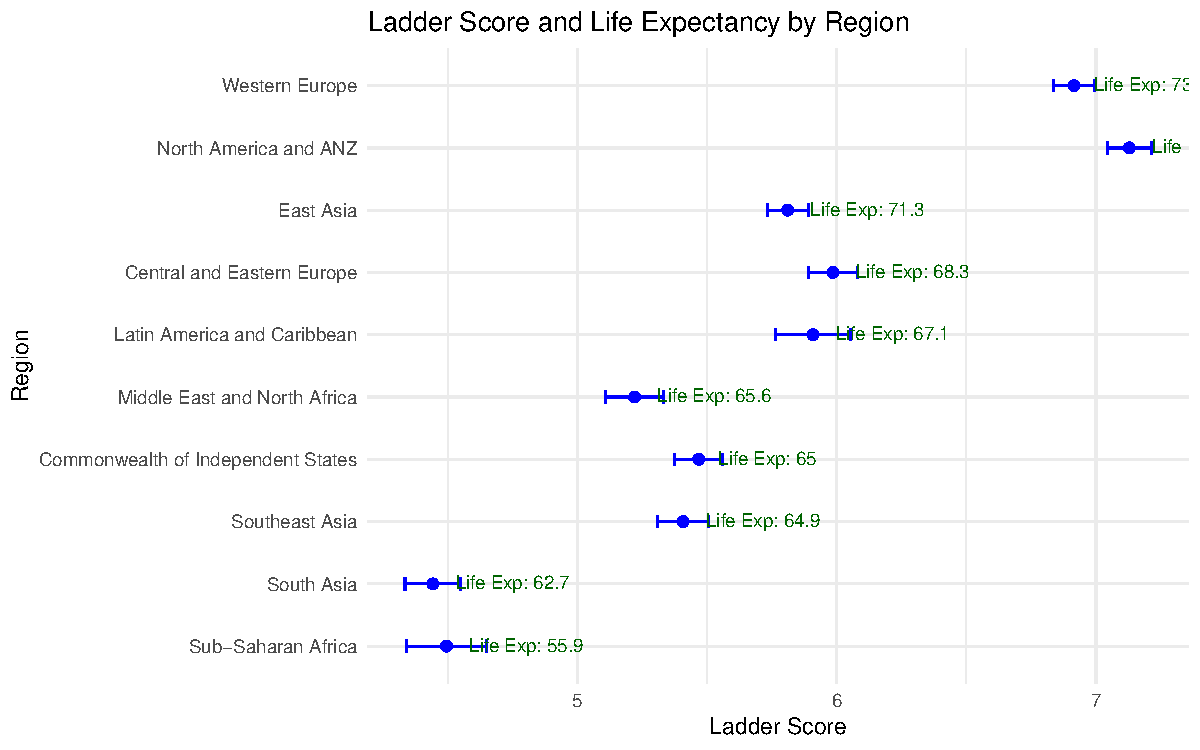
\includegraphics{23084103_HAPPINESS_files/figure-latex/unnamed-chunk-3-1.pdf}
The graph displays average Ladder Scores (a proxy for life satisfaction)
across world regions, with horizontal error bars showing upper and lower
confidence intervals. Regions like Western Europe, North America \& ANZ,
and East Asia report the highest Ladder Scores, suggesting greater
average happiness levels. In contrast, Sub-Saharan Africa and South Asia
rank lowest. Above each region, the corresponding Healthy Life
Expectancy is labeled --- regions with higher life expectancy tend to
also report higher happiness scores. This visual supports the notion
that health outcomes are closely associated with subjective well-being.
The ordering of regions by life expectancy helps highlight this pattern
clearly.

1b)

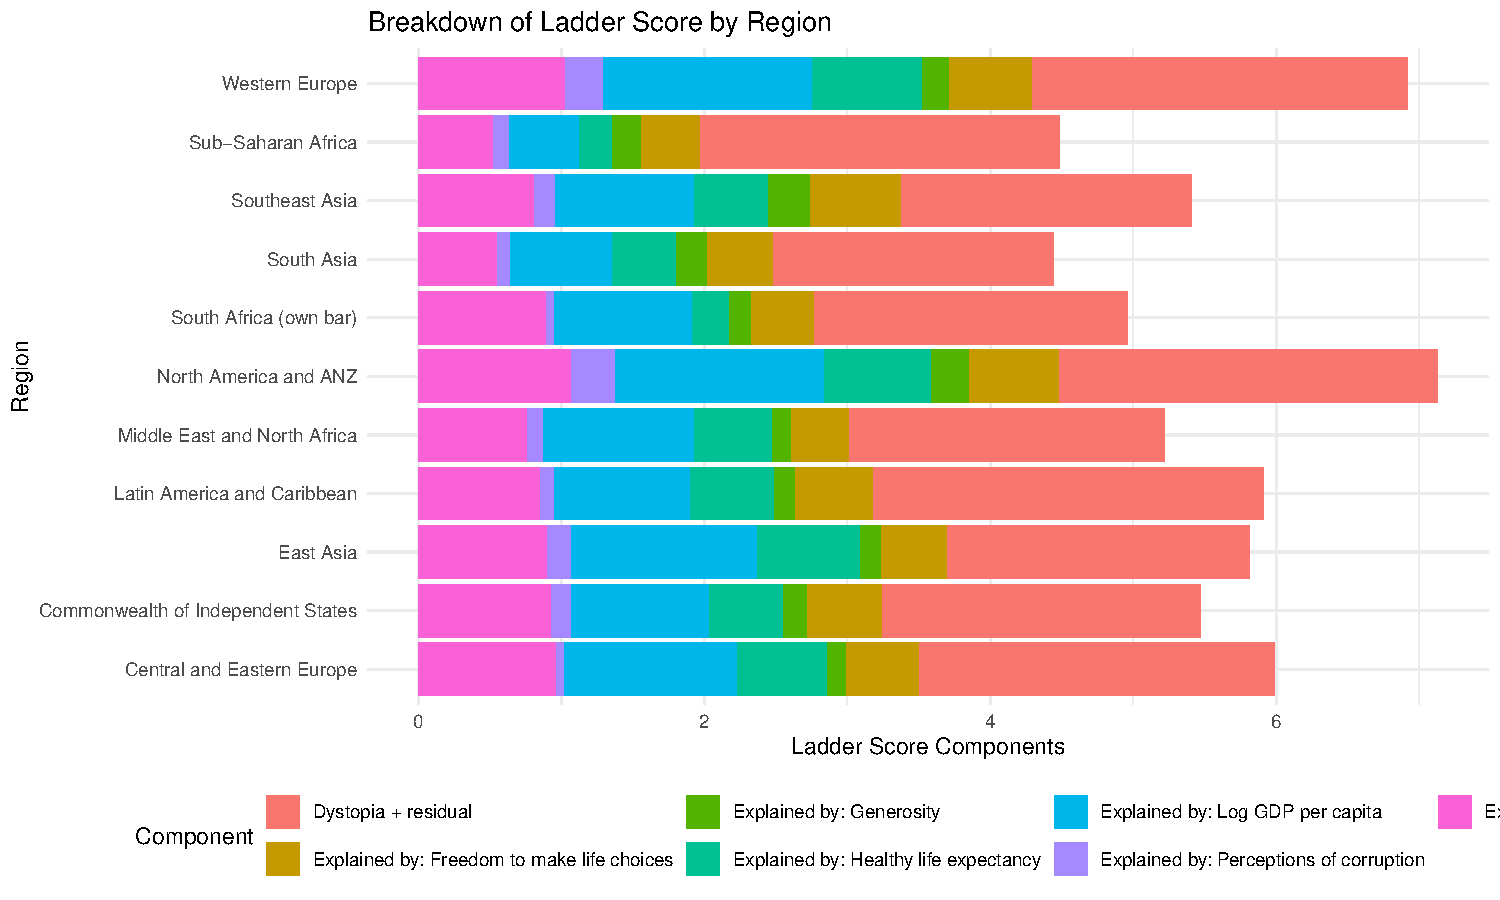
\includegraphics{23084103_HAPPINESS_files/figure-latex/unnamed-chunk-4-1.pdf}
The plot shows the composition of the Ladder Score across global
regions, broken down into components like social support, generosity,
and residuals. Western Europe and North America lead with the highest
scores, driven by strong contributions from GDP and social support.
South Africa's bar (added manually) appears prominently, with a high
contribution from ``Dystopia + residual,'' indicating significant
unexplained happiness. In contrast, regions like Sub-Saharan Africa and
South Asia show lower scores, largely due to smaller contributions from
economic and institutional factors. The comparison reveals wide
disparities in the structural sources of well-being across the globe.

\section{Conclusion}\label{conclusion}

The analysis reveals that Healthy Life Expectancy strongly correlates
with higher life satisfaction scores across regions. Regions like
Western Europe and North America show both high ladder scores and long
life expectancies, while Sub-Saharan Africa lags in both. South Africa
stands out with a relatively high Ladder Score compared to its region,
largely driven by residuals and social support. The stacked barplot
breakdown emphasizes that non-economic factors such as freedom and
social trust play a vital role. This suggests that money alone does not
guarantee happiness. Investments in health and well-being infrastructure
may yield better outcomes for life satisfaction. Overall, happiness is
multifaceted and context-dependent.

\bibliography{Tex/ref}





\end{document}
